\newpage
\section{Problem 3: WARM-UP}\label{problem-3-warm-up}
Original image \cref{fig3} for question \textbf{(a)} \& \textbf{(b)}.
\begin{figure}
    \centering
    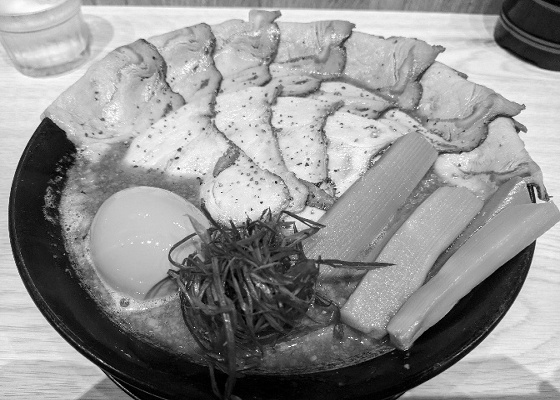
\includegraphics[width=0.7\textwidth]{image/sample5.jpg}
    \caption{\textbf{sample5.jpg}}
    \label{fig3}
\end{figure}

% a
\textbf{(a)} Design proper filters to remove noise from \textbf{sample6.jpg} and \textbf{sample7.jpg}, and output the resultant images as \textbf{8\_result.jpg} and \textbf{9\_result.jpg}, respectively. 
Please detail the {\textbf{steps} of the denoising process and specify all the \textbf{corresponding parameters}}. Provide some discussions about the reason why those filters and parameters are chosen.

\subsection{Uniform noise}
\textbf{Motivation}
For \textbf{sample6.jpg} \cref{fig3u}, this is \textbf{uniform noise}.
\begin{figure}
    \centering
    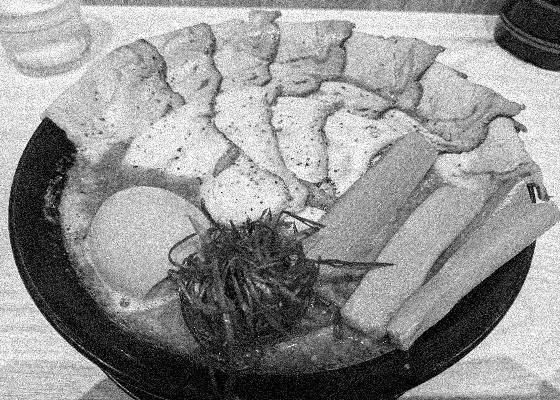
\includegraphics[width=0.7\textwidth]{image/sample6.jpg}
    \caption{\textbf{sample6.jpg}}
    \label{fig3u}
\end{figure}

We could follow the \textbf{low-pass filtering} strategy in \textit{Lec 2 page 22}.

\textbf{Approach}
My approach is based on \textbf{low-pass filtering}.
\begin{enumerate}
    \item Given \emph{kernel size}~\(k=5\) \& \emph{scalar (b)}\(=2\) as parameters of \textbf{convolution matrix}.
    \item Expand the \textbf{image array} accroding to \emph{kernel\_size}~\(k=5\). In practice, expand boundary with \(2=\lfloor \frac{5}{2} \rfloor\).
    \item Create the \textbf{convolution matrix}:\\
    I build it with \textbf{cross-}\(b\) patterns:
    \begin{equation}
      \frac{1}{(b + k - 1)^{2}}
      \begin{bmatrix}
        1 & \dots & b & 1 & \dots & 1 \\
        \vdots & \ddots & b & \vdots & \ddots & 1 \\
        b & \dots & b^{2} & b & \dots & b \\
        1 & \dots & b & 1 & \dots & 1 \\
        \vdots & \ddots & b & \vdots & \ddots & \vdots \\
        1 & \dots & b & 1 & \dots & 1
      \end{bmatrix}
    \end{equation}
    e.g. for $k=5$, $b=2$
    \begin{equation}
      \frac{1}{(2 + 5 - 1)^{2}}
      \begin{bmatrix}
        1 & 1 & 2 & 1 & 1 \\
        1 & 1 & 2 & 1 & 1 \\
        2 & 2 & 2^{2} & 2 & 2 \\
        1 & 1 & 2 & 1 & 1 \\
        1 & 1 & 2 & 1 & 1
      \end{bmatrix}
    \end{equation}
    \item Collect the \textbf{sub arrays} from \textbf{expanded image array}.
    \item Conduct the \textbf{convolution/weighted average} by \textbf{convolution matrix} on each \textbf{sub arrays}.
\end{enumerate}

\textbf{Performance of results}
Result of problem 3(a): \textbf{8\_result.jpg} with $\mbox{PSNR}=30.9034$ \cref{fig3a_1}.
\begin{figure}
    \centering
    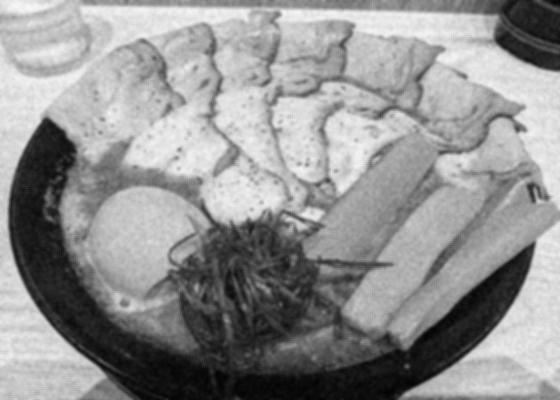
\includegraphics[width=0.7\textwidth]{image/8_result.jpg}
    \caption{\textbf{8\_result.jpg} Low-pass filter on uniform noise}
    \label{fig3a_1}
\end{figure}

\textbf{Discussion}
A little foggy. But it's fine to me.
And we can see \textbf{meidan filter on uniform noise} \cref{fig3a_1m} is similar to \textbf{loss-pass filter}. Its PSNR is $30.1825$ not far from \textbf{8\_result.jpg} ($30.9034$). I consider that the \textbf{real pepper} bring about the good discriminative features.
\begin{figure}
  \centering
  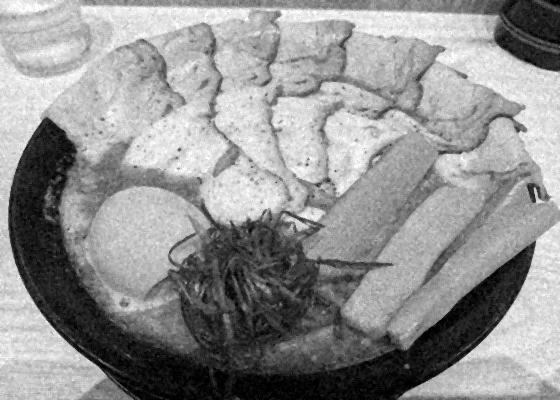
\includegraphics[width=0.7\textwidth]{image/tmp/8_result_median.jpg}
  \caption{Median filter on uniform noise}
  \label{fig3a_1m}
\end{figure}

\subsection{Impulse noise}
\textbf{Motivation}
For \textbf{sample7.jpg} \cref{fig3i}, this is \textbf{impulse noise}.
\begin{figure}
  \centering
  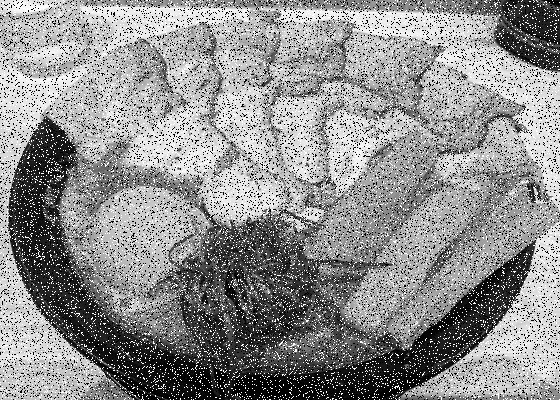
\includegraphics[width=0.7\textwidth]{image/sample7.jpg}
  \caption{\textbf{sample7.jpg}}
  \label{fig3i}
\end{figure}
We could follow the \textbf{median filtering} strategy in \textit{Lec 2 page 22}.

\textbf{Approach}
My approach is based on \textbf{median(percentile) filtering}. 
\begin{enumerate}
    \item Given \emph{kernel size}~\(k=3\) \& \emph{percentile (percent)}\(=50\) (Note \(50\)\% is just the \emph{median}.) as parameters.
    \item Expand the \textbf{image array} accroding to \emph{kernel\_size}~\(k=3\). In practice, expand boundary with \(1=\lfloor \frac{3}{2} \rfloor\).
    \item Collect the \textbf{sub arrays} from \textbf{expanded image array}.
    \item Calculate the $50$\textbf{-th percentile} on each \textbf{sub arrays}.
\end{enumerate}
To get the better result, I conduct the \textbf{median filtering} \alert{twice} again on the origin image.

\textbf{Performance of results}
Result of problem 3(a): \textbf{9\_result.jpg} with $\mbox{PSNR}=33.0975$ \cref{fig3a_2}.
\begin{figure}
  \centering
  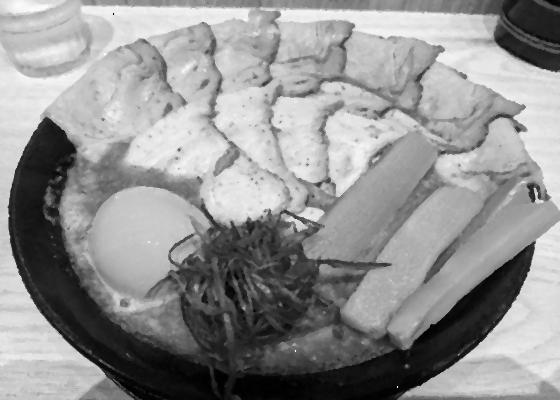
\includegraphics[width=0.7\textwidth]{image/9_result.jpg}
  \caption{\textbf{9\_result.jpg} Median filter on impulse noise}
  \label{fig3a_2}
\end{figure}

\textbf{Discussion}
Awesome! We get a beautiful \textit{egg}. :-)

And we can see \textbf{low-pass filter on uniform noise} \cref{fig3a_2l} is not good. Its PSNR is $28.4716$ less than \textbf{9\_result.jpg} ($\mbox{PSNR}=33.0975$).
\begin{figure}
  \centering
  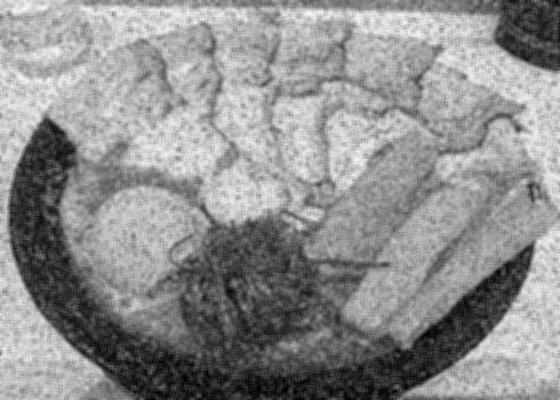
\includegraphics[width=0.7\textwidth]{image/tmp/9_result_low_pass.jpg}
  \caption{Low-pass filter on impulse noise}
  \label{fig3a_2l}
\end{figure}

\textbf{(b)} Compute the PSNR values of \textbf{8\_result.jpg} and \textbf{9\_result.jpg} and provide some discussions.

\textbf{Motivation}
As we have the original image as the \alert{ground truth}, we could design the \textbf{metric} to evaluate how well we denoise. 

\textbf{Approach}
Based on \textbf{Peak signal-to-noise ratio, PSNR} in \textit{Lec 2 page 38}.
\begin{equation}
\mbox{PSNR} = 10 \times \log_{10} \left(\frac{255^{2}}{\mbox{MSE}}\right)
\end{equation}
where \(\mbox{MSE}\) is
\begin{equation}
\mbox{MSE} = \frac{1}{w \times h}\sum_{j}\sum_{k}\left[F(j, k) - F^{\textnormal{\textquotesingle}}(j, k) \right]^{2}
\end{equation}

\textbf{Performance of results}
Result of problem 3(b): For \textbf{8\_result.jpg}, it's PSNR is \alert{30.9034}.
We could see that we eliminate uniform noise/fogging but vaguer than the original image.

Result of problem 3(b): For \textbf{9\_result.jpg}, it's PSNR is \alert{33.0975}.
We could see that we eliminate impulse noise/salt and pepper. But some \textbf{real pepper} are also disappeared. And a little vague than the original image.

\textbf{Discussion}
Note: We could find out that \textbf{once-time median filter on impulse noise} as \cref{fig3b_once}. Its PSNR is \textbf{33.0480}. It has more pepper but the region at \textbf{egg} is still dirty. So I choose the latter one.
\begin{figure}
\centering
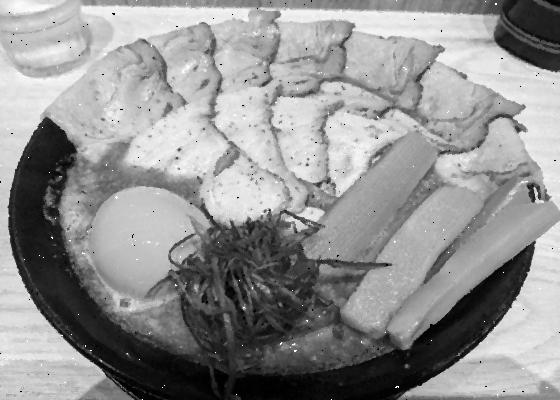
\includegraphics[width=0.7\textwidth]{image/tmp/9_result_once.jpg}
\caption{once-time median filter on impulse noise}
\label{fig3b_once}
\end{figure}

\textbf{Analysis of parameters}
As we have \textbf{PSNR} metric to evaluate how well we denoise/recover to the original image. We could observe the relationship between parameters and PSNR.

\textbf{Low-pass filter on uniform noise}
For \textbf{sample6.jpg (low-pass filter)}, we observe the parameters kernel size $k$ \cref{fig3_6k} \& scalar $b$ \cref{fig3_6b}.
\begin{figure}
  \centering
  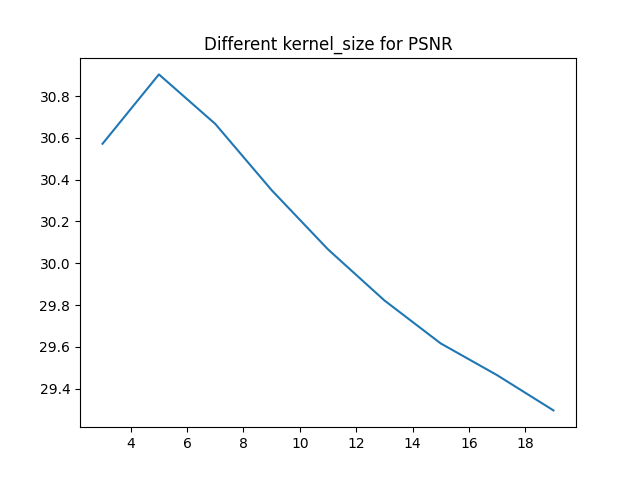
\includegraphics[width=0.7\textwidth]{image/sample6_paramkernel_size.png}
  \caption{\textbf{Analysis of kernel size $k$}}
  \label{fig3_6k}
\end{figure}
\begin{figure}
  \centering
  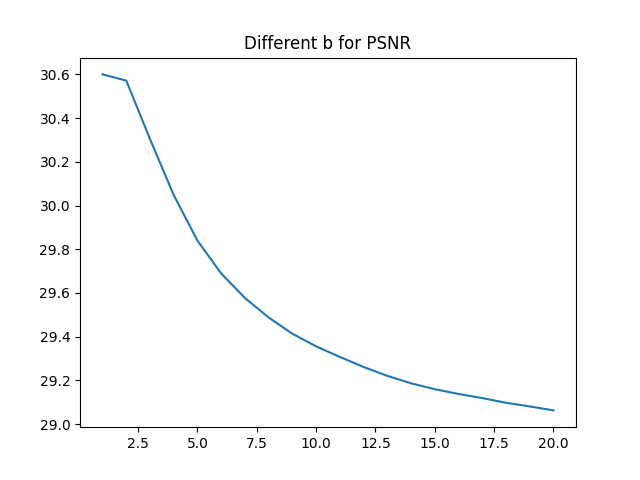
\includegraphics[width=0.7\textwidth]{image/sample6_paramb.png}
  \caption{\textbf{Analysis of scalar $b$}}
  \label{fig3_6b}
\end{figure}
And we could see the \textbf{best PSNR} occurs at $b=2$ \& $k=5$.

Note: I don't conduct \textbf{grid search} as it spends a lot of time.

\textbf{Median filter on impulse noise}
For \textbf{sample7.jpg (meidan filter)}, we observe the parameters kernel size $k$ \cref{fig3_7k} \& percentile $p$ \cref{fig3_7p}.
\begin{figure}
  \centering
  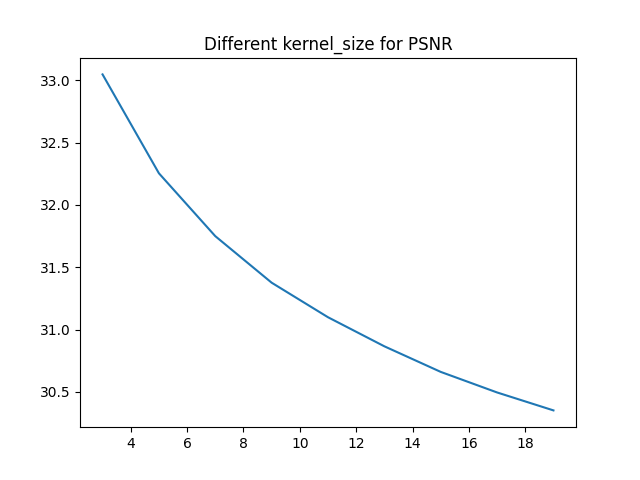
\includegraphics[width=0.7\textwidth]{image/sample7_paramkernel_size.png}
  \caption{\textbf{Analysis of kernel size $k$}}
  \label{fig3_7k}
\end{figure}
\begin{figure}
  \centering
  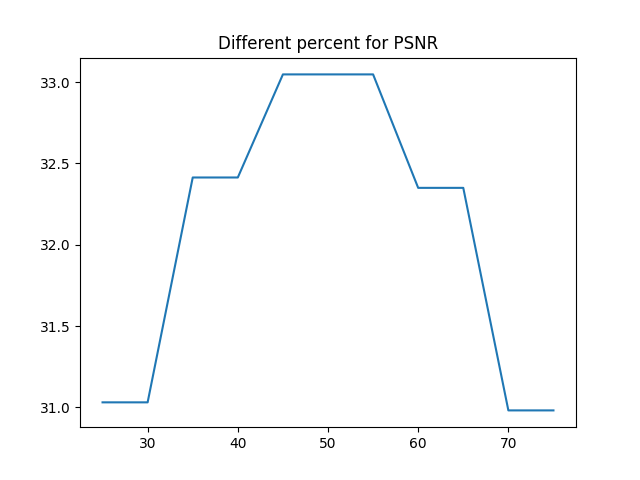
\includegraphics[width=0.7\textwidth]{image/sample7_parampercent.png}
  \caption{\textbf{Analysis of percentile $p$}}
  \label{fig3_7p}
\end{figure}
And we could see the \textbf{best PSNR} occurs at $k=3$ \& $p=50$ (median).

% ------------------------------------------------------------------------
\subsection{Denoise by Fast Fourier Transform (FFT) on uniform noise}

\textbf{Motivation}
As Amy says we could try denoise in the frequency domain by FFT.

We could see the distribution of intensity in the frequency domain looks uniform. Both on \textbf{uniform noise} \cref{fig3_8fft_orig}.
\begin{figure}
  \centering
  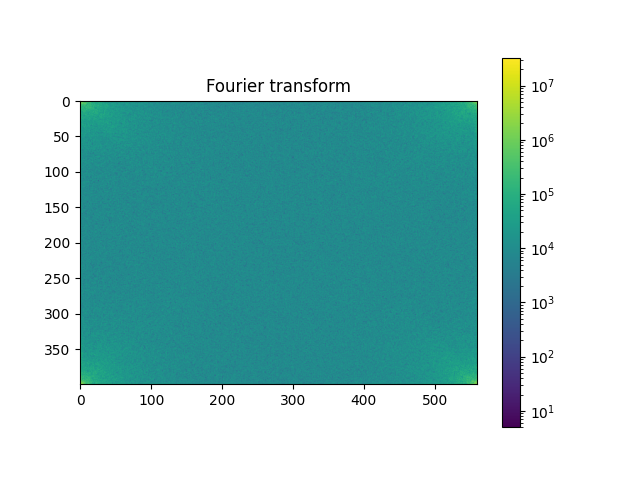
\includegraphics[width=0.7\textwidth]{image/tmp/sample6_FD_origin.png}
  \caption{\textbf{frequency domain of \textbf{sample6.jpg}}}
  \label{fig3_8fft_orig}
\end{figure}
If we keep $10$\% signal in the frequency domain. We can obtain the result \cref{fig3_8fft} with a little less PSNR than \textbf{low-pass filter} ($30.9034$). Its PSNR is $30.1494$.
\begin{figure}
  \centering
  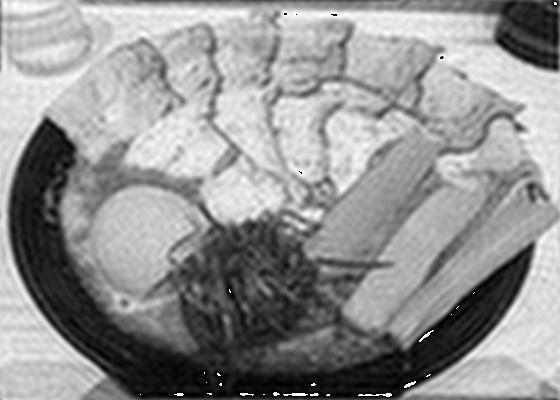
\includegraphics[width=0.7\textwidth]{image/tmp/8_result_fft.jpg}
  \caption{\textbf{frequency domain of \textbf{sample6.jpg}}}
  \label{fig3_8fft}
\end{figure}
